\documentclass[a4paper,twoside]{book}

\usepackage[utf8]{inputenc}
\usepackage[english,russian]{babel}
\usepackage{graphicx}
\usepackage{hyperref}
\usepackage{multirow}
\usepackage[absolute,overlay,showboxes]{textpos}
\usepackage{etoolbox}
\usepackage{longtable}
\usepackage{tikz}

\urlstyle{same}
\usepackage[printonlyused,withpage]{acronym}

\graphicspath{ {images/} }

%% This procedure adds the "Example" block to the text.
\newcommand{\example}[1]{
  \fbox {
    \textbf{Пример:}
    \parbox{\linewidth}{#1}
  }
}

\newcommand{\note}[1]{
  \fbox {
    \textbf{Примечание:}
    \parbox{\linewidth}{#1}
  }
}

\newcommand{\hotkey}[1]{
  \texttt{#1}
}

%% This procedure allows to insert a music note.
%% Syntax:
%%   \musicnote{<octave>}{<note-name>}{<frequency>}
\newcommand{\musicnote}[3]{
  &
  \ifstrequal{#2}{C}{До   & C#1}{}
  \ifstrequal{#2}{D}{Ре   & D#1}{}
  \ifstrequal{#2}{E}{Ми   & E#1}{}
  \ifstrequal{#2}{F}{Фа   & F#1}{}
  \ifstrequal{#2}{G}{Соль & G#1}{}
  \ifstrequal{#2}{A}{Ля   & A#1}{}
  \ifstrequal{#2}{B}{Си   & B#1 (H#1)}{}
  & #3 \\
}

\title{Автоматопрограмматокомпарадиокружок}
\author{Артём ``avp'' Попцов}
\date{\today}

\begin{document}

\maketitle

\tableofcontents

\chapter{Начало пути}

\section{Добро пожаловать!}

Дорогой читатель, добро пожаловать в наш уютный кружок технического творчества.
Здесь мы учимся работать со звуком, светом, электричеством, используя наши
знания для создания неожиданных, интересных и практически полезных проектов. Мы
постараемся сделать ваш путь в мир электроники и программирования как можно
более интересным и лёгким. Но и на вас лежит определённая отвественность --
во-первых, без вашего активного участия наши усилия могут не дать желаемого
эффекта. Во-вторых, мы учимся вместе с вами, и ты, уважаемый читатель, являешься
активным участником работы над этой книгой. Если найдёшь ошибки или опечатки, не
стесняйся писать нам по указанным в книге контактам -- мы постаремся всё
исправить в следующей версии книги.

Надеемся, что данная станет вашей настольной (или хотя бы \emph{около-стольной},
но во всяком случе не \emph{под-стольной}) книгой, которая поможет постичь
искусство программирования и отчасти исследовать и возможно понять мир вокруг
нас немного лучше, чем вы понимали прежде.

\section{Для кого предназначена данная книга?}
Вы открыли первую страницу книги и задаётесь вопросом -- а стоит ли эта книга
времени, которое будет потрачено на её чтение? К сожалению, вынуждены вас
огорчить -- данную книгу нужно будет не только читать, но и прилагать некоторые
усилия для освоения материала. Как будто собираясь в поход, вы должны
подготовиться и взять с собой необходимые вещи. Но не торопитесь закрывать на
этом книгу -- мы можем предложить вам то, ради чего вы возможно захотите пройти
весь путь до конца. Во-первых, где-то на горизонте, в манящей доступности,
располагаются диковинные земли, до которых вы можете дойти и изучить их, узнав
много нового. Во-вторых, поход будет хоть и не самым простым, но зато подарит
вам массу впечатлений, опыта -- и быть может даже будущую профессию.

\section{Авторы}
В разработке данной книги принимали участие следующие люди:
\begin{itemize}
\item Денис Киселёв -- вклад в разработку отдельных глав книги; вычитка текста,
  участие в разработке и тестирование примеров, приведённых в книге.
\item Сергей Ермейкин -- вычитка текста, исправление ошибок.
\item Илья Маштаков – вычитка и доработка текста.
\end{itemize}

\section{Лицензия}
Copyright © 2016-2022 Артём ``avp'' Попцов.

Права на копирование сторонних изображений и материалов, использованных в данной
работе, принадлежат их владельцам.

Данная работа распространяется на условиях лицензии
«Attribution-NonCommercial-ShareAlike» («Атрибуция — Некоммерческое
использование — На тех же условиях») 4.0 Всемирная (CC BY-NC-SA 4.0):
\url{https://creativecommons.org/licenses/by-nc-sa/4.0/deed.ru}

\chapter{Знакомство с набором разработки Arduino}

\section{Введение}
По нашему мнению, программирование является двоякой дисциплиной: с одной
стороны, это – один из видов творчества, позволяющий человеку создать что-то
необычное, новое и, возможно, полезное для общества; с другой стороны, это –
инструмент, позволяющий решать практические, прикладные задачи. Как кисти и
краски художника, или инструменты музыканта, инструменты программиста имеют
большое разнообразие в видах и применениях. Чтобы освоить их в полной мере
требуются годы. Тем не менее, долгий путь начинается с первого шага.

Данная книга позволяет людям, желающим освоить программирование, сделать первый
шаг на пути в профессии программиста. Вам предлагается изучить основы
программирования на C, разрабатывая приложения для платформы Arduino.

\section{Работа с макетной платой}

Макетная плата позволяет собирать схемы (подключать электронику) без применения
пайки --- это упрощает прототипирование и ускоряет процесс разработки проектов.
Компоненты просто вставляются в слоты на макетной плате для соединения.

\begin{itemize}
\item Черный провод подключен к arduino и идёт на вывод GND (минус)
\item Синий провод подключен к arduino и идёт на вывод 5V (плюс)
\end{itemize}

\emph{Примечание:} обратите внимание, что светодиоды (и некоторые другие
элементы) подключаются к платформе Arduino через резистор -- это необходимо для
обеспечения бесперебойной работы схемы и предупреждения всяческих поломок и
ухудшения работы как отдельных деталей, так и схемы в целом.

\section{Подключение Arduino к компьютеру}
Чтобы подключить ардуино к компьютеру вам потребуется сама платформа Arduino (в
нашем случае мы используем Arduino Mega 2560) и кабель стандарта USB-В.

Соедините Arduino с компьютером через USB-кабель. Вы увидите, как на плате
загорится светодиод «ON».

Теперь необходимо настроить Arduino IDE для работы с подключенной Arduino, для
этого нужно войти в панель “Инструменты” затем “Плата” -- в этом меню выберите
6Arduino с которой вы сейчас работаете, затем в подменю “Порт” выберите порт, к
которому подключена Arduino.

\section{Знакомство со средой разработки Arduino}
Среда разработки Arduino (Arduino IDE) состоит из встроенного текстового
редактора программного кода, области сообщений, окна вывода текста (консоли),
панели инструментов с кнопками часто используемых команд и нескольких меню. Для
загрузки программ и связи с компьютером среда разработки подключается к
аппаратной части Arduino.

Скачать среду разработки можно с официального сайта Arduino:
\url{https://www.arduino.cc/en/Main/Software}.

Перед скачиванием будет предложено пожертвовать денег проекту Arduino для
дальнейшего развития, но этот шаг необязателен и может быть выполнен на ваше
усмотрение.

Ниже приведено описание кнопок в интерфейсе Arduino IDE.

\begin{tabular}{p{4cm}|p{6cm}}
  Название & Описание \\
  \hline \hline
  Verify/Compile (Проверка) & Проверка программного кода. \\
  \hline
  Upload (Загрузка) & Компилирует программный код.\\
  \hline
  New (Создать) & Создание нового скетча.\\
  \hline
  Open (Открыть) & Открыть скетч.\\
  \hline
  Save (Сохранить) & Сохранить скетч.\\
  \hline
  Serial Monitor (Монитор порта) & Открыть монитор порта.\\
\end{tabular}

\section{Основы работы с мультиметром}
Мультиметр -- незаменимый прибор, с его помощью можно узнать сопротивление
резистора, измерить напряжение, произвести проверку на проводимость
(``прозвонка''), узнать цвет и полярность светодиода и многое другое.

Далее приведена таблица на которой отражены основные символы, встречающиеся на
корпусе прибора, необходимые для работы с мультиметром:


\section{Структура программы на Arduino}

Программа для Arduino обычно состоит из двух основных частей, также называемых
функциями: "setup" и "loop". Пример программы, которая мигает одним светодиодом:
\begin{verbatim}
void setup() {
    pinMode(2, OUTPUT);
}

void loop() {
    digitalWrite(2, HIGH);
    delay(500);
    digitalWrite(2, LOW);
    delay(500);
}
\end{verbatim}

Функция \texttt{setup} производит инициализацию микроконтроллера при его
включении. В неё следует помещать все команды, которые должны выполняться
единожды на старте системы.

Цифровой порт (или, по-другому, пин) Arduino может находиться в двух состояниях.
В режиме входа пин считывает напряжение, а в режиме выхода – позволяет выдавать
на пине такое же напряжение.

Рассмотрим приведённый выше пример. В \texttt{setup} выполняется функция
\texttt{pinMode}, которая позволяет настроить режим работы указанного пина как
вход или выход:

\begin{verbatim}
  pinMode(pin, mode);
\end{verbatim}

где \texttt{pin} -- номер пина, \texttt{mode} -- режим работы
(\texttt{INPUT}/\texttt{OUTPUT}).

В \texttt{loop} вызываются две функции: \texttt{digitalWrite} и \texttt{delay}.

Функция
\begin{verbatim}
  digitalWrite(pin,value);
\end{verbatim}

где \texttt{pin} -– номер пина, \texttt{value} -- уровень сигнала
(\texttt{HIGH}/\texttt{LOW}), подаёт на пин высокое или низкое напряжение.

Функция
\begin{verbatim}
delay(value);
\end{verbatim}

где \texttt{value} -- количество миллисекунд, останавливает выполнение программы
на указанное время.

\subsection{Задачи}
\begin{itemize}
\item Соберите на макетной плате ``бегущий огонь'': светодиоды должны поочерёдно
  включаться и выключаться, один за другим.
\item Модифицируйте ``бегущий огонь'' так, чтобы он бежал сначала в одну
  сторону, затем в другую.
\end{itemize}

\section{Переменные и память}

\emph{Переменная} -- это ключевое понятие в программировании. Любая программа
работает с данными. Возьмём для наглядности некую программу- калькулятор,
умеющую складывать два числа. Чтобы микроконтроллер мог работать с этими числами
их нужно где-то хранить. Где? В оперативной памяти. Все данные, которые
используются микроконтроллером во время работы, хранятся именно там. Для работы
нашего калькулятора нужно загрузить в ячейки оперативной памяти два
числа-операнда, которые нужно сложить, например 15 и 3:

\begin{tabular}{p{4cm}|p{6cm}}
  Адрес ячейки & Значение ячейки \\
  \hline \hline
  0000 & 15 \\
  \hline
  0001 & 3 \\
  \hline
  0003 & 0 \\
  ... & ... \\
\end{tabular}

\emph{Переменная} -- это ячейка данных в оперативной памяти (ОЗУ). Объявить
переменную –- значит сказать компьютеру выделить какую-нибудь ячейку памяти для
наших нужд.

Переменная в языке С++ имеет определённый тип и уникальное имя. Объявление
(\emph{инициализация}) переменной выглядит следующим образом:

\begin{verbatim}
тип имя = значение;
\end{verbatim}

То есть, чтобы загрузить в оперативную память два числа 15 и 3, мы должны написать
следующее:

\begin{verbatim}
int a = 15;
int b = 3;
\end{verbatim}

Слово \texttt{int} это тип переменной, означает, что эта переменная является
числом.

Также следует объявить переменную для хранения результата сложения:

Дальше -- складываем значения двух переменных \texttt{a} и \texttt{b}:

\begin{verbatim}
int result = a + b;
\end{verbatim}

Здесь мы присвоили переменной \texttt{result} результат операции сложения двух
переменных.

\emph{ВАЖНО!} Имя переменной может состоять только из букв, цифр и нижнего
подчёркивания, причём имя не может начинаться с цифры.

Вернёмся к нашим светодиодам. Объявим новую переменную:

\begin{verbatim}
int k = 500;
\end{verbatim}

Что мы можем с ней сделать? Например, в программе мигания светодиодом заменим ею
значение задержки в функции \texttt{delay}. Вообще, переменным следует давать
осмысленные имена, в нашем случае пусть это будет не \texttt{k}, а
\texttt{delay\_val}:

\begin{verbatim}
void loop() {
    int delay_val = 500;
    digitalWrite(2, HIGH);
    delay(delay_val);
    digitalWrite(2, LOW);
    delay(delay_val);
}
\end{verbatim}

Таким образом, мы сможем поменять значения всех задержек одной заменой значения
\texttt{delay\_val}:

\begin{verbatim}
void loop() {
    int delayVal = 600;
    // ...
}
\end{verbatim}

Можно, например, увеличивать \texttt{delay\_val} на 100 при каждом выполнении
\texttt{loop}:

\begin{verbatim}
void loop() {
    int delay_val = 100;
    12digitalWrite(2, HIGH);
    delay(delay_val);
    digitalWrite(2, LOW);
    delay(delay_val);
    delay_val = delay_val + 100;
}
\end{verbatim}

Кстати, строчку \texttt{delay\_val = delay\_val + 100} можно заменить на
\texttt{delay\_val += 100} и результат будет тем же, но запись короче.

\texttt{+=} -- оператор присваивания, совмещённый со сложением.

Существуют также другие операторы подобного рода -- например, ``-=''
(читается ``минус-равно'') Если мы запустим этот код, то увидим, что задержка
переключения светодиодов… не меняется. Почему? При каждом выполнении loop()
каждый раз объявляется новая переменная \texttt{delay\_val} со значением 100 и
потому задержка остаётся той же. Сейчас delayVal объявлена как локальная
переменная внутри \texttt{loop}, следует объявить её за пределами функции, чтобы
она стала глобальной:

\begin{verbatim}
int delay_val = 100;

void loop() {
  digitalWrite(2, HIGH);
  delay(delay_val);
  digitalWrite(2, LOW);
  delay(delay_val);

  delay_val += 100;
}
\end{verbatim}

Теперь всё будет работать. Но так задержка будет бесконтрольно расти. Решением
будет сделать так, чтобы \texttt{delay\_val} увеличивалась до какого-то
порогового значения, например, до 600. Для этого нужно добавить условие
(\texttt{if}):

\begin{verbatim}
int delay_val = 100;

void loop() {
    digitalWrite(2, HIGH);
    delay(delay_val);
    digitalWrite(2, LOW);
    delay(delay_val);

    if (delay_val < 600){
      delay_val += 100;
    }
}
\end{verbatim}

Об условиях и других управляющих конструкциях -- в следующей главе.

\chapter{Управляющие конструкции языка C++}

\section{Условия}

Иногда во время выполнения программы следует принять решение о том, что делать
дальше. Для того, чтобы компьютер мог сделать правильный выбор, по какому пути
пойти, нам, как программистам, следует описать условия в коде программы: если
условие выполняется, делаем одно, иначе -- делаем другое.

Условия в программах описываются при помощи специальных управляющих конструкций.
В языке C++ у нас есть две основные конструкции. Первая из них -- оператор
\texttt{if} (буквально в переводе с английского ``если''). Пример использования:

\begin{verbatim}
if (a > 10) {
    // действие, выполняемое, если значение
    // переменной 'a' больше 10.
}
\end{verbatim}

Если нужно проверить равно ли значение переменной чему-либо, используют оператор
сравнения ``=='':

\begin{verbatim}
if (a == 10) {
    // действие, выполняемое, если значение
    // переменной 'a' равно 10.
}
\end{verbatim}

Не путайте оператор сравнения ``=='' с оператором присваивания ``='' - это важно!

Часто необходимо не только делать что-либо при выполнении условия, но и
предоставить альтернативную инструкцию (или набор инструкций), выполняемую
тогда, когда условие не выполняется. В этом случае используют конструкцию
\texttt{if ... else}:

\begin{verbatim}
if (a > 10) {
  // действие, выполняемое, если значение
  // переменной 'a' больше 10.
} else {
  // действие, выполняемое, если значение
  // переменной 'a' меньше или равно 10.
}
\end{verbatim}

Второй оператор, который нам будет встречаться, это так называемый
\emph{оператор выбора} \texttt{switch}. С ним познакомимся позже. Он удобен,
например, тогда, когда нам нужно выполнять несколько разных действий в
зависимости от значения переменной, и этих действий много.

\section{Циклы}

Простые программы, вроде ``бегущего огня'', могут быть написаны простым
копированием и вставкой алгоритма мигания светодиода (возможно, с небольшими
модификациями).

А теперь представьте, что вам требуется запрограммировать ``бегущий огонь'' на
100 светодиодов. Утомительная задача, не правда ли? Для того, чтобы не делать
тупую работу по копированию одного и того же кода много раз, программистами
придуманы специальные управляющие конструкции, называемые \emph{циклами}.

Циклы бывают разные. Основные виды циклов, которые вам будут встречаться
практически в любом языке программирования:
\begin{itemize}
\item Цикл со счётчиком (также называемый ``параметрический цикл'').
\item Цикл с предусловием.
\item Цикл с постусловием.
\end{itemize}

Каждый вид циклов имеет собственную реализацию в языке программирования, который
мы используем (C++).

\subsection{Цикл со счётчиком}

Цикл со счётчиком реализуется конструкцией \texttt{for} -- она позволяет нам
создать счётчик, задать его начальное значение, описать условие выполнения цикла
и операцию изменения счётчика:

\begin{verbatim}
//                   5.
//        1.         2.           4.
for (int pin = 0; pin < 10; pin = pin + 1) {
    // 3. (тело цикла)
}
\end{verbatim}

Выполняется эта конструкция в следующем порядке:
\begin{enumerate}
\item объявляем переменную и присваиваем ей значение 0 (шаг 1);
\item переходим к проверке, где смотрим, выполняется ли условие (шаг 2);
\item после этого, если условие 2 выполняется, мы переходим к телу цикла (шаг 3);
\item после выполнения тела цикла, мы переходим к изменению значения счётчика (шаг 4);
\item после шага 4 мы опять возвращаемся к шагу 2, если условие выполняется, то
  переходим к шагу 3 и т.д.
\end{enumerate}

\subsection{Цикл с предусловием}

Другим распространённым видом цикла является цикл с предусловием, реализуемый в
С++ конструкцией \texttt{while} -- данный вид цикла удобен в тех случаях, когда
мы не знаем точного количества раз, сколько нужно повторить тело цикла (не знаем
количество итераций.)

Общий вид цикла \texttt{while} таков:
\begin{verbatim}
int pin = 2;

while (pin < 10) {
    // тело цикла
}
\end{verbatim}

\subsection{Цикл с постусловием}

Кроме вышеперечисленных видов циклов, есть ещё цикл с постусловием, где
проверка условия выполнения цикла осуществляется после выполнения тела цикла.
Реализуется данный вид циклов конструкцией \texttt{do..while}.

Он достаточно редкоиспользуется и мы не будем на нём здесь останавливаться.

\subsection{Зачем столько видов циклов?}

Обратите внимание, что один вид цикла может быть реализован через другой, т.к.
данные управляющие конструкции взаимозаменяемы. Возникает вопрос -- зачем же
16нам нужно столько видов циклов? Всё дело в удобстве. В одних случаях удобнее
использовать один вид циклов, в других случаях -- другой.

У программистов есть специальный термин для описания подобных конструкций языка
программирования: синтаксический сахар. Синтаксический сахар -- это конструкции
языка, без которых в принципе можно обойтись при разработке программ, но с ними
всё проще ("слаще").

\subsection{Задачи}
\begin{enumerate}
\item Перепишите ``бегущий огонь'' с использованием цикла.
\item Модифицируйте алгоритм ``бегущего огня'' таким образом, чтобы светодиоды
  начинали загораться с обоих концов гирлянды и огни ``бежали'' навстречу друг
  другу.
\end{enumerate}

\chapter{Широтно-импульсная модуляция}

\section{Общее описание принципов работы}

Широтно-импульсная модуляция, или сокращённо \emph{ШИМ}, позволяет выдавать на
цифровом порту Arduino напряжение в диапазоне от 0 до 5 вольт, используя при
этом только два сигнала -- \texttt{HIGH} (логическая единица, при которой на
порт подается 5 В) и \texttt{LOW} (логический ноль, при котором на порт подается
0 В.) Меняя быстро данные значения на порту, можно добиться, например,
напряжения в 2.5 В.

\section{Длина волны}

При создании ``мигающего светодиода'' мы попеременно подавали на цифровой порт
сигналы \texttt{HIGH} и \texttt{LOW}, с указанием задержки (в миллисекундах).
Если мы посмотрим на вид сигнала на цифровом порту во времени (скажем, с помощью
осциллографа), то увидим примерно следующую картину:


Где \emph{длина периода} -- расстояние между двумя ближайшими друг к другу
точками в пространстве, в которых колебания происходят в одинаковой фазе.

Зная длину периода, можно рассчитать \emph{частоту колебаний}, и наоборот --
зная частоту, можно рассчитать длину волны.

При работе с ШИМ мы будем использовать длину периода, заданную в микросекундах
(мкс). 1 микросекунда -- это одна миллионная часть секунды. Для краткости записи
подобных маленьких величин часто используется возведение числа 10 в
отрицательную степень. Ниже приведена таблица с указанием различных долей
секунды\footnote{Для полного списка кратных и дольных единиц см. статью
\href{https://ru.wikipedia.org/wiki/\%D0\%A1\%D0\%B5\%D0\%BA\%D1\%83\%D0\%BD\%D0\%B4\%D0\%B0}{Секунда}
в Википедии.}:

\begin{tabular}{p{4cm}|p{4cm}|p{6cm}}
  Название & Величина & Пример \\
  \hline \hline
  секунда (с) & $ 1 с $ или $ 10^0 с $ & $ 500 * 10^{0} = 500 с $ \\
  \hline
  миллисекунда (мс) & $ 0.001 c $ или $ 10^{-3} c $ & $ 500 * 10^{-3} = 500 мс $ \\
  \hline
  микросекунда (мкс) & $ 0.000001 c $ или $ 10^{-6} c $ & $ 500 * 10^{-6} = 500 мкс $ \\
  \hline
  наносекунда (нс) & $ 0.000000001 c $ или $ 10^{-9} с $ & $ 500 * 10^{-9} = 500 нс $
\end{tabular}

\section{Коэффициент заполнения}

Каким образом задается напряжение из диапазона? Очень просто: путём изменения
времени подачи того или иного сигнала. Чем больше времени на порту сигнал HIGH,
тем выше напряжение. При этом, длина периода \texttt{P} остаётся фиксированной
(например, 1000 микросекунд). Таким образом для ШИМ важно процентное отношение
одного сигнала к другому, и, увеличивая время подачи одного сигнала, следует
уменьшать время подачи другого (следовательно если мы подаем сигнал
\texttt{HIGH} 60\% от отведенного времени, нужно заполнить оставшиеся 40\%
сигналом \texttt{LOW}).

Отношение периода следования сигнала к длительности импульса называется
\emph{скважностью}. В англоязычной литературе величина, обратная скважности,
называется \emph{коэффициентом заполнения} (англ. \emph{duty cycle}).

Мы будем использовать термин ``коэффициент заполнения''.

\example {
  Мы хотим получить 2.5 вольта на цифровом порту 2, имея в
  распоряжении только два значения -- 0 В и 5 В. Для этого нам потребуется
  реализовать ШИМ с коэффициентом заполнения 50\%. При длине волны в 1000
  микросекунд мы должны половину времени (500 микросекунд) заполнить
  положительным сигналом (сигнал \texttt{HIGH}) и подать его на выбранный порт, затем
  остальную часть заполним отрицательным сигналом (сигналом \texttt{LOW}).
  Если всё сделано правильно, то на 2 цифровом порту получим 2.5 вольта.
}

Для генерации нужного сигнала нам потребуется создать инструмент
(\emph{функцию}), который впоследствии мы будем использовать. Мы уже говорили о
важности написания и использования собственных функций в программе -- функции
позволяют нам создавать модульные программы, упрощают поддержку существующего
программного кода и написание нового кода.

Подумаем над тем, какой должна быть наша функция, реализующая ШИМ. Ниже приведён
знакомый нам график, отображающий сигнал на цифровом порту -- мы будем
использовать этот график, как основу для написания функции.

%% TODO: Add the graph.

В программе мы обозначим длину периода константой \texttt{P}, равной 1000 мкс.
Значения задержек, заданных переменными \texttt{d1} и \texttt{d2}, необходимо
вычислить на основе коэффициента заполнения, задаваемого параметром функции
\texttt{duty\_cycle} (который задаётся дробным значением -- к примеру, 0.5.)

Имея перед глазами этот график, нетрудно набросать словесное описание функции
(назовём функцию \texttt{pwm}, как сокращение от англ. \emph{pulse width
  modulation}.)

Начнём с того, что, скорее всего, подобная функция должна принимать три
параметра:
\begin{enumerate}
\item Номер порта (обозначаемый целым числом), на котором следует сгенерировать
  ШИМ сигнал; назовём этот параметр \texttt{pin}.
\item Коэффициент заполнения, заданный дробным числом -- к примеру, 50\% будет
  задано, как 0.5; назовём этот параметр \texttt{duty\_cycle}
\item Длина ШИМ сигнала в микросекундах; назовём этот параметр
  \texttt{signal\_length}.
\end{enumerate}

Запишем тоже самое на языке С++:

\begin{verbatim}
void pwm(int pin, float dc, long signal_length) {
  // тело функции
}
\end{verbatim}

О том, что такое \texttt{void}, будет сказано позже, пока что стоит принять как
факт, что это начало объявления функции. Наверняка появились вопросы по новым
типам переменных -- \texttt{float} и \texttt{long}. Почему нельзя использовать
привычный \texttt{int}? Дело в том, что переменная типа \texttt{int} не может
хранить дробные числа, а также имеет диапазон значений от -32 768 до 32 767. Для
хранения дробных чисел используется \texttt{float}, а для чисел, не входящих в
диапазон \texttt{int}, стоит использовать \texttt{long}, имеющий диапазон от -2
147 483 648 до 2 147 483 647. Теперь подумаем над телом функции. Первым делом
нам необходимо задать константу \texttt{P}:

\begin{verbatim}
const int P = 1000; // мкс
\end{verbatim}

Обратите внимание, что мы используем ключевое слово const для того, чтобы
пометить \texttt{WAVE\_LENGTH}, как константу -- мы всё равно не собираемся
менять это значение. Кроме того, мы указали в комментарии, что значение задано в
микросекундах (мкс), что упрощает чтение кода. В C++, да и в других языках,
константа -- это та же переменная, но её значение нельзя менять после её
объявления.

Следующим этапом будет вычисление в теле функции значений переменных \texttt{d1}
и \texttt{d2} на основе значения \texttt{duty\_cycle}, заданного при вызове
функции:

\begin{verbatim}
int d1 = P * duty_cycle;
int d2 = P - d1;
\end{verbatim}

Видно, что как только мы вычислили \texttt{d1}, вычислить \texttt{d2} не
составляет труда. Осталось только посчитать, сколько раз нужно повторить волну
длиной \texttt{P}, чтобы сгенерировать сигнал длиной \texttt{signal\_length}:

\begin{verbatim}
int count = signal_length / P;
\end{verbatim}

Теперь у нас есть всё, что нужно для генерации нужного нам сигнала. Поскольку
исходя из описания выше нам нужно будет повторять волну count раз, то для этого
удобно использовать цикл \texttt{for} (цикл со счётчиком):

\begin{verbatim}
for (int c = 0; c < count; c++) {
  digitalWrite(pin, HIGH);
  delayMicroseconds(d1);
  digitalWrite(pin, LOW);
  delayMicroseconds(d2);
}
\end{verbatim}

Готово! Осталось только задействовать функцию pwm в нашей программе.

\subsection{Задачи}

\begin{enumerate}
\item Написать программу, плавно включающую и выключающую светодиод. Собрать и
  протестировать схему. 
\item Написать программу, реализующую ``бегущий огонь'' с использованием ШИМ.
  Собрать и протестировать схему.
\item Используя потенциометр, модифицировать систему из задания №2 таким
  образом, чтобы можно было регулировать яркость ``бегущего огня''.
\item Разработать ``бегущий огонь'', где следующий светодиод начинает плавно
  разгораться одновременно с затуханием предыдущего светодиода.
\end{enumerate}

\section{Использование потенциометра}

Поставим себе задачу -- вручную регулировать скорость ``бегущего огня'' в
реальном времени. Микроконтроллер должен принимать извне некий сигнал, величину
которого мы можем регулировать каким-либо элементом управления и использовать в
качестве параметра:

\begin{verbatim}
Сигнал -> Элемент управления -> Arduino -> Параметр
\end{verbatim}

Для считывания сигнала можно использовать аналоговые порты Arduino. На плате они
подписаны как \texttt{A0}, \texttt{A1}, и т.д. Если цифровые порты рассчитаны на
цифровой сигнал, который может быть в двух состояниях - 0 В или 5 В, то
аналоговые, соответственно, рассчитаны на аналоговый, непрерывный, сигнал,
который может принимать любые значения от 0 до 5 В.

Микроконтроллер измеряет напряжение на аналоговом порту и преобразовывает
полученное значение в число от 0 до 1023, которое мы можем использовать для
своих нужд.

В качестве элемента управления может служить такой компонент как потенциометр.
Переменный резистор или потенциометр -- это резистор, сопротивление которого,
как понятно из названия, можно изменять. Используя потенциометр, мы можем влиять
на поступающее напряжение на порт, тем самым регулируя нужный нам параметр.
Подключаем крайние выводы потенциометра к питанию и земле, а центральный -- к
аналоговому порту.

В коде будем использовать функцию \texttt{analogRead}:

\begin{verbatim}
int value = analogRead(A0); // Получаем значение с аналогового порта 0
\end{verbatim}

\texttt{A0} - номер аналогового порта. Функция \texttt{analogRead} возвращает
результат вышеописанной операции -- число от 0 до 1023.

Осталась одна проблема -- нам неизвестно значение, которое получил
микроконтроллер. Для этого воспользуемся последовательным портом.

\section{Последовательный порт}

Последовательный порт в Arduino -- это тот самый USB-B, который мы подключаем
всякий раз, когда желаем включить наш микроконтроллер или загрузить в Arduino
какую-либо программу. С помощью последовательного порта можно передавать данные
с Arduino на компьютер и наоборот.

\subsection{Основы работы с Arduino через последовательный порт}

Прежде, чем начать работать с последовательным портом, нам необходимо его
настроить; делается это следующим образом: в теле функции setup мы должны
написать:

\begin{verbatim}
Serial.begin(9600);
\end{verbatim}

В этом случае мы обеспечиваем обмен данными между компьютером и Arduino с
указанной скоростью, где 9600 -- это скорость, с которой мы передаем данные на
персональный компьютер в \emph{бодах} (битах в секунду.) Обычно данный параметр
принимает одно из следующих значений: 300, 600, 1200, 2400, 4800, 9600, 14400,
19200, 28800, 38400, 57600, 115200.

\subsection{Передача данных с Arduino на компьютер}

Теперь попробуем передать данные с аналогового порта Arduino на компьютер. В
качестве примера мы просто отправим строку ``Hello, world!'' по
последовательному порту. Для начала пропишем настройку порта в функции
\texttt{setup}:

\begin{verbatim}
void setup() {
  Serial.begin(9600); // устанавливаем скорость порта
}
\end{verbatim}

А вот так в нашем случае выглядит функция \texttt{loop}:

\begin{verbatim}
void loop() {
  int value = analogRead(0); // Получаем данные с аналогового порта

  // отправляем переменную value с помощью
  // последовательного порта:
  Serial.println(value);

  delay(100); // ждём 100 мс перед следующей отправкой
}
\end{verbatim}

Результат выполнения программы можно увидеть, открыв монитор порта в Arduino
IDE. Доступ к монитору порта можно получить, нажав кнопку в виде лупы в правом
верхнем углу редактора кода:

Кроме того, открыть монитор порта можно, нажав комбинацию клавиш \hotkey{Ctrl +
  Shift + M}. Также можно использовать плоттер по последовательному соединению,
который выводит графики поступающих данных. Чтобы его открыть, нужно перейти во
вкладку ``Инструменты'' $\rightarrow$ ``Плоттер по последовательному
соединению'':

\subsection{Использование монитора порта для отладки программ}

Передачу данных с Arduino на компьютер можно использовать в множестве разных
задач. Примером одной из таких задач является простейший способ отладки программ
-- с помощью вывода информации о работе программы в Arduino на последовательный
порт. Иными словами, вместо того, чтобы пытаться самим понять, что же пошло не
так и почему что-то не работает, мы просим Arduino саму рассказывать нам, что
она делает.

\subsection{Сбор и обработка данных на стороне компьютера}

Другой задачей, решаемой с помощью функций записи данных в последовательный
порт, является сбор данных на стороне компьютера. Arduino IDE позволяет нам
визуализировать данные через специальный плоттер (доступ к которому можно
получить, выбрав в меню ``Инструменты'' пункт ``Плоттер по последовательному
соединению'', либо нажав комбинацию клавиш \hotkey{Ctrl + Shift + L}.)

\subsection{Передача данных с компьютера на Arduino}

Передавать данные с Arduino на компьютер мы уже научились. Теперь посмотрим на
передачу данных в обратном направлении. Для того чтобы передать данные с
компьютера на Arduino также необходимо выполнить настройку последовательного
порта; кроме этого, нам потребуется задействовать несколько новых функций.

\subsubsection{Чтение отдельных байт}

Функция \texttt{Serial.read} читает байт данных из поступивших на Arduino. То
есть возвращает вам некое целое число, с которым вы вольны делать что вашей душе
угодно. Каждый вызов этого метода будет возвращать вам следующий байт данных из
тех что поступили на Arduino. Если возвращать нечего, то есть вы считали все что
было, данная функция вернет -1.

\note{ Если передаются именно байты, возникает проблема: -1 это 0xFF в
  шестнадцатиричной системе, или 255 в десятичной. Такой же байт, как и все
  остальные, из-за чего невозможно. поэтому нужно сперва вызывать функцию available . }

Допустим мы отправили 1 байт данных на Arduino и использовали нижеприведенный
участок кода:

\begin{verbatim}
int incoming_byte;
void loop() {
  if (Serial.available() > 0) {
      incoming_byte = Serial.read();
  }
}
\end{verbatim}

После того, как вы считаете байт данных, он будет перемещен в вашу переменную
\texttt{incoming\_byte} а функция \texttt{Serial.available} снова будет
возвращать 0, пока не поступят новые данные.

То есть, когда вы считываете байт, показания счетчика принятых байт уменьшается
и \texttt{Serial.available} будет показывать на 1 байт меньше.

Помните, что функция \texttt{Serial.read} возвращает только 1 байт данных, если
например вы передали 4 символа каждый по 1 байту, вам потребуется 4 раза вызвать
данную функцию чтобы прочитать эти символы и самостоятельно позаботится о том
чтобы разместить их в массив символов либо воспользоваться функцией
\texttt{Serial.readBytes}.

\subsubsection{Чтение чисел}

Функция \texttt{Serial.parseInt} просматривает данные, поступившие на Arduino, и
ищет среди них набор кодов (чисел) от 48 до 57, которые соответствуют символам
чисел от 0 до 9 и преобразует все это в правильное целочисленное значение. Таким
образом если вы с монитора порта передадите "число" (на самом деле, строку)
``72'', данный метод увидит 2 последовательных байта 55 и 51, корректно
преобразует его в число 72 и вернет его как правильное целочисленное значение.
Давайте напишем маленькую эхо-программу, которая покажет принцип работы данной
функции и позволит вам узнать какому символу соответствует то или иное число.

\begin{verbatim}
int incoming_int = 0;

void setup()
{
  Serial.begin(9600);
  Serial.setTimeout(2000);
}
void loop()
{
  if (Serial.available() > 0)
  {
    incoming_int = Serial.parseInt();
    Serial.write(incoming_int);
  }
}
\end{verbatim}

Данная программа будет работать так. Если в мониторе порта вы введете строку
``72'' то монитор порта отправит его на Arduino как два байта данных в виде
чисел 55 и 51, функция \texttt{Serial.parseInt} подождет 2000 миллисекунд (как
видите я поменял время ожидание с 1 секунды на 2 секунды, чтобы нагляднее
показать кое какие аспекты) увидит эти два значения и преобразует их в одно
целочисленное 72 и присвоит его переменной \texttt{incoming\_int}, мы с помощью
метода \texttt{Serial.write} передадим число 72 как есть обратно в монитор порта
(почему именно этот метод нужен читайте далее) где монитор порта корректно
преобразует число 72 в соответствующий символ и покажет нам символ ``H'' который
соответствует коду 72. Таким образом мы можем передавать числовые значения с
компьютера на платформу Arduino и дальше использовать эти значения.

\chapter{Аналогово-цифровое преобразование}

Чтобы не терялась нить повествования, в главе ``Использование потенциометра''
стоило умолчать о том, как Arduino проводит преобразование напряжения с
аналогового порта в дискретное значение от 0 до 1023. Задавшись вопросом -- ``А
почему именно 1023?'', мы сможем познакомиться с такой интересной штукой как
АЦП. \emph{Аналого-Цифровой Преобразователь} (АЦП) - это устройство, которое и
проводит преобразование.

Преобразование проходит в три этапа:
\begin{enumerate}
\item \emph{Дискретизация.} Выбираются значения из исходного аналогового сигнала через
  равные временные промежутки (\ref{fig:discretization}.)

  \begin{figure}[h]
    \caption{Дискретизация.}
    \label{fig:discretization}
    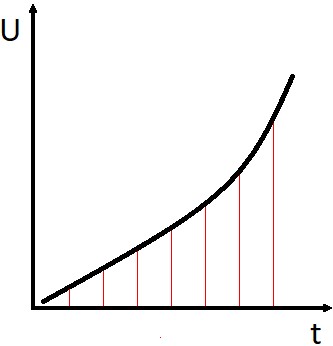
\includegraphics[width=8cm]{discretization}
    \centering
  \end{figure}

  Характеристика, отражающая эти временные промежутки, называется частота
  дискретизации.
\item \emph{Квантование.} Полученные значения заменяются ближайшим значением из
  набора фиксированных величин -- \emph{уровней квантования}
  (\ref{fig:quantization}.)

  \begin{figure}[h]
    \caption{Квантование.}
    \label{fig:quantization}
    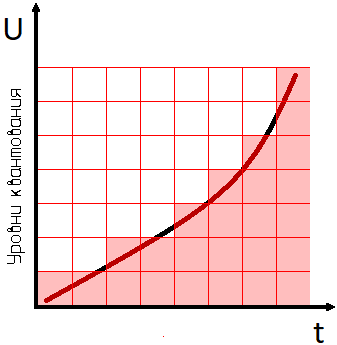
\includegraphics[width=8cm]{quantization}
    \centering
  \end{figure}

\item \emph{Кодирование.} Квантованным значениям присваивается цифровой код
  (\ref{fig:coding}.)

  \begin{figure}[h]
    \caption{Кодирование.}
    \label{fig:coding}
    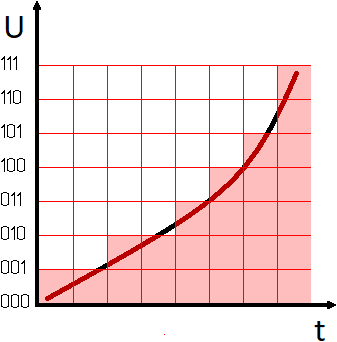
\includegraphics[width=8cm]{coding}
    \centering
  \end{figure}

  Чем выше частота дискретизации и чем больше уровней квантования, тем точнее
  преобразование.

\end{enumerate}

Одной из характеристик АЦП является \emph{разрядность}. Она определяет
количество значений, которое может выдать АЦП. Посмотрим на последний график:
для кодирования значений используется три бита, значит АЦП, описываемый таким
графиком, имеет, соответственно, разрядность 3 бита. То есть $ 2^3 = 8 $, что
равно количеству уровней квантования.

Вот и ответ на поставленный вопрос. АЦП Arduino 10-ти разрядный, $2^10 = 1024$.
Именно столько значений АЦП Arduino может выдать.

Ещё есть такое устройство как ЦАП - \emph{Цифро-Аналоговый Преобразователь},
который, как нетрудно догадаться, выполняет функцию, обратную функции АЦП -
преобразует цифровой сигнал в аналоговый. Область применения ЦАП и АЦП
достаточно широка: в звуковых и видео- картах, в мониторах, в различной
акустической аппаратуре, в измерительных приборах, и многих других видах
техники.

Стоит упомянуть про 8-битную музыку в древних игровых консолях. Её название
отражает разрядность ЦАП звуковых чипов тех консолей -- 8 бит. Именно такой ЦАП
позволял выдавать тот самый резковатый, хлопающий и шипящий звук.

\chapter{Синтез музыки и технологии}

\section{Звук}

Как известно \emph{звук} -- это колебания (вид сигнала), и каждому определённому
звуку соответствует своя частота колебаний.

Частоты измеряются в \emph{Герцах} (Гц), и один Герц (1 Гц) означает одно
колебание в секунду. 10 колебаний в секунду -- 10 Гц, 100 колебаний в секунду --
100 Гц и т. д. Если же мы говорим про частоты в 100 Гц и более, то удобнее
использовать приставки Кило- (КГц), Мега- (МГц) и Гига- (ГГц): сигнал с частотой
1 КГц поданный на цифровой порт колеблет мембрану динамика 1000 раз в секунду.
Ниже приведена таблица некоторых кратных единиц частот в Герцах:

\begin{tabular}{p{3cm}|p{4cm}|p{3.5cm}}
  Название & Величина & Пример \\
  \hline \hline
  Герц (Гц)
  & $ 1 \mbox{Гц} $ или $ 10^0 \mbox{Гц} $
  & $ 100 * 10^0 \mbox{Гц} = 100 \mbox{Гц} $ \\
  \hline
  Килогерц (КГц)
  & $ 1000 \mbox{Гц} $ или $ 10^3 \mbox{Гц} $
  & $ 100 * 10^3 \mbox{Гц} = 1 \mbox{КГц} $ \\
  \hline
  Мегагерц (МГц)
  & $ 1000000 \mbox{Гц} $ или $ 10^6 \mbox{Гц} $
  & $ 100 * 10^6 \mbox{Гц} = 1 \mbox{МГц} $ \\
  \hline
  Гигагерц (ГГц)
  & $ 1000000000 \mbox{Гц} $ или $ 10^9 \mbox{Гц} $
  & $ 100 * 10^9 \mbox{Гц} = 1 \mbox{ГГц} $ \\
\end{tabular}

Таким образом, для генерации сигнала нам необходимо знать его частоту в Герцах,
либо знать длину волны.

Зная период, мы можем узнать частоту, и наоборот -- поскольку частота является
ничем иным, как количеством повторений заданных колебаний в секунду. Это удобно
представить визуально (\ref{fig:sound-fig-1}.)

\begin{figure}[h]
  \caption{Визуальное представление частоты колебаний 5 Гц.}
  \label{fig:sound-fig-1}
  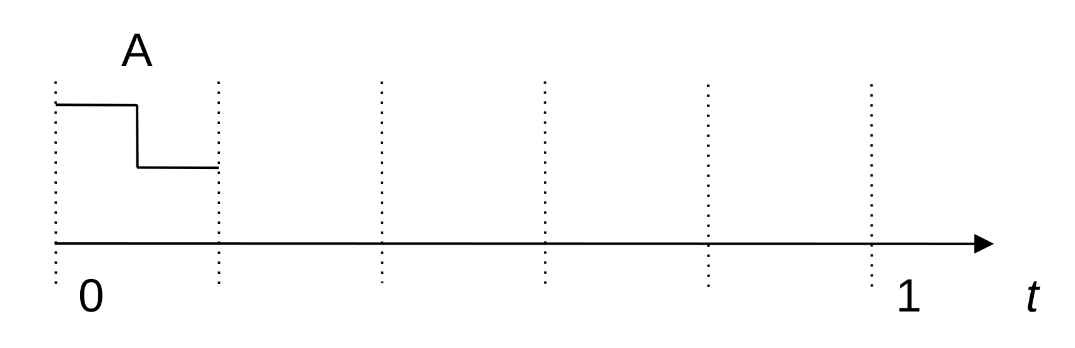
\includegraphics[width=10cm]{sound-fig-1}
  \centering
\end{figure}

Если известно, что колебание А помещается 5 раз в 1 секунду, то говорят, что
частота данного сигнала равна 5 Гц. Узнать период можно, разделив 1 секунду
(заданную в микросекундах) на частоту (5 Гц):

\begin{equation}
  \frac{1000000 \mbox{мкс}}{5 \mbox{Гц}} = 200000 \mbox{мкс}
\end{equation}

Получается, что длина волны равна 200000 мкс, или $ 200 * 10^3 \mbox{мс} $. Если
же нам известна длина волны и нужно узнать частоту, то необходимо разделить 1
секунду (в микросекундах) на длину волны -- таким образом, получим частоту в
Герцах. Всё просто.

Метод генерации звука похож на ШИМ. Основные отличия заключаются в том, что
теперь мы должны изменять длину волны len, оставляя коэффициент заполнения
неизменным -- он описывается константой DC и всегда равен 0.5. Поскольку
коэффициент заполнения всегда равен 50\% (0.5), то время подачи сигналов
\texttt{HIGH} и \texttt{LOW} всегда одинаково -- иными словами, нам достаточно
вычислить только задержку \texttt{d1}. Это показано на графике ниже:

Как и в случае с ШИМ, начнём писать функцию, которая будет реализовывать
вышеописанные принципы. Функция будет называться \texttt{play\_tone} и будет
позволять генерировать звук с нужной частотой на указанном цифровом порту.

Посмотрим, что данная функция должна принимать в качестве параметров:
\begin{enumerate}
\item Номер цифрового порта, к которому подключен динамик и куда будет
  выводиться звук; назовём этот параметр ``pin'';
\item Частота ``f'', измеряемая в Герцах. 
\item Длина звукового сигнала; назовём этот параметр ``t''.
\end{enumerate}

На языке C++ это будет выглядеть примерно так:
\begin{verbatim}
void play_tone(int pin, float f, long t) {
    // тело функции
}
\end{verbatim}

Теперь пришло время написать тело функции. Начнём с того, что зададим
коэффициент заполнения в виде константы:
\begin{verbatim}
const float DC = 0.5; // 50%
\end{verbatim}

Теперь из частоты найдём период \texttt{p}:
\begin{verbatim}
long p = 1000000 / f;
\end{verbatim}

Далее посчитаем длину задержки \texttt{d}:
\begin{verbatim}
int d = p * DC;
\end{verbatim}

И посчитаем, сколько раз нам нужно повторить период длиной p микросекунд, чтобы
заполнить время \texttt{t}:
\begin{verbatim}
int count = t / p;
\end{verbatim}

Почти всё готово. Осталось только написать цикл, который будет генерировать
заданную волну нужное количество раз. Здесь отлично подойдёт цикл со счётчиком
(\texttt{for}):

\begin{verbatim}
for (int c = 0; c < count; c++) {
  digitalWrite(pin, HIGH);
  delayMicroseconds(d);
  digitalWrite(pin, LOW);
  delayMicroseconds(d);
}
\end{verbatim}

В общем виде, функция выглядит так:

\begin{verbatim}
void play_tone(int port, float f, long t) {
  const int T = 1000000 / f;
  int d = T / 2;
  int count = t / T;
  for (int i = 0; i < count; i++) {
    digitalWrite(port, HIGH);
    delayMicroseconds(d);
    digitalWrite(port, LOW);
    delayMicroseconds(d);
  }
}
\end{verbatim}

Наша функция генерации звука завершена. Теперь нам нужно подключить динамик к
Arduino и протестировать нашу систему.

\note{Во многих случаях одна и та же задача может быть решена несколькими
  способами. К примеру, функция \texttt{play\_tone} может быть реализована
  иначе; предложенная нами реализация является только одной из корректных. Как
  вариант, вы можете реализовать вариант функции, которая оперирует не длиной
  волны, а частотой. Подумайте над этим в свободное время. И не бойтесь
  экспериментировать! }

%%%%%%%%%%%%%%%%%%%%%%%%%%%%%%%%%%%%%%%%%%%%%%%%%%%%%%%%%%%%%%%%%%%%%%%%%%%%%%%%
\section{Подключение динамика}

Есть несколько вариантов динамиков, которые вы можете встретить. Например, есть
обычные динамики, где мембрана колеблется магнитным полем и тем самым создаёт
колебания воздуха, которые мы слышим, как звук. Есть пьезодинамики, в которых
звук генерируется за счёт обратного пьезоэлектрического эффекта -- механической
деформации пьезоэлектрика под действием электрического поля.\footnote{См. статью
"Пьезоэлектрический эффект" в Википедии для более подробного описания эффекта.}

Подключение и обычных динамиков и пьезодинамиков похоже; для наших задач
подойдёт как пьезодинамик ``для Arduino'', так и обычный динамик-пищалка из
персонального компьютера (а вы знали, что у вас в компьютере к системной плате
подключен динамик?)

Схема подключения представлена на рис. \ref{fig:sound-fig-2}.

%% TODO: Перерисовать схему.  Убрать резистор.
\begin{figure}[h]
  \caption{Подключение динамика-''пищалки'' к Arduino Mega 2560.}
  \label{fig:sound-fig-2}
  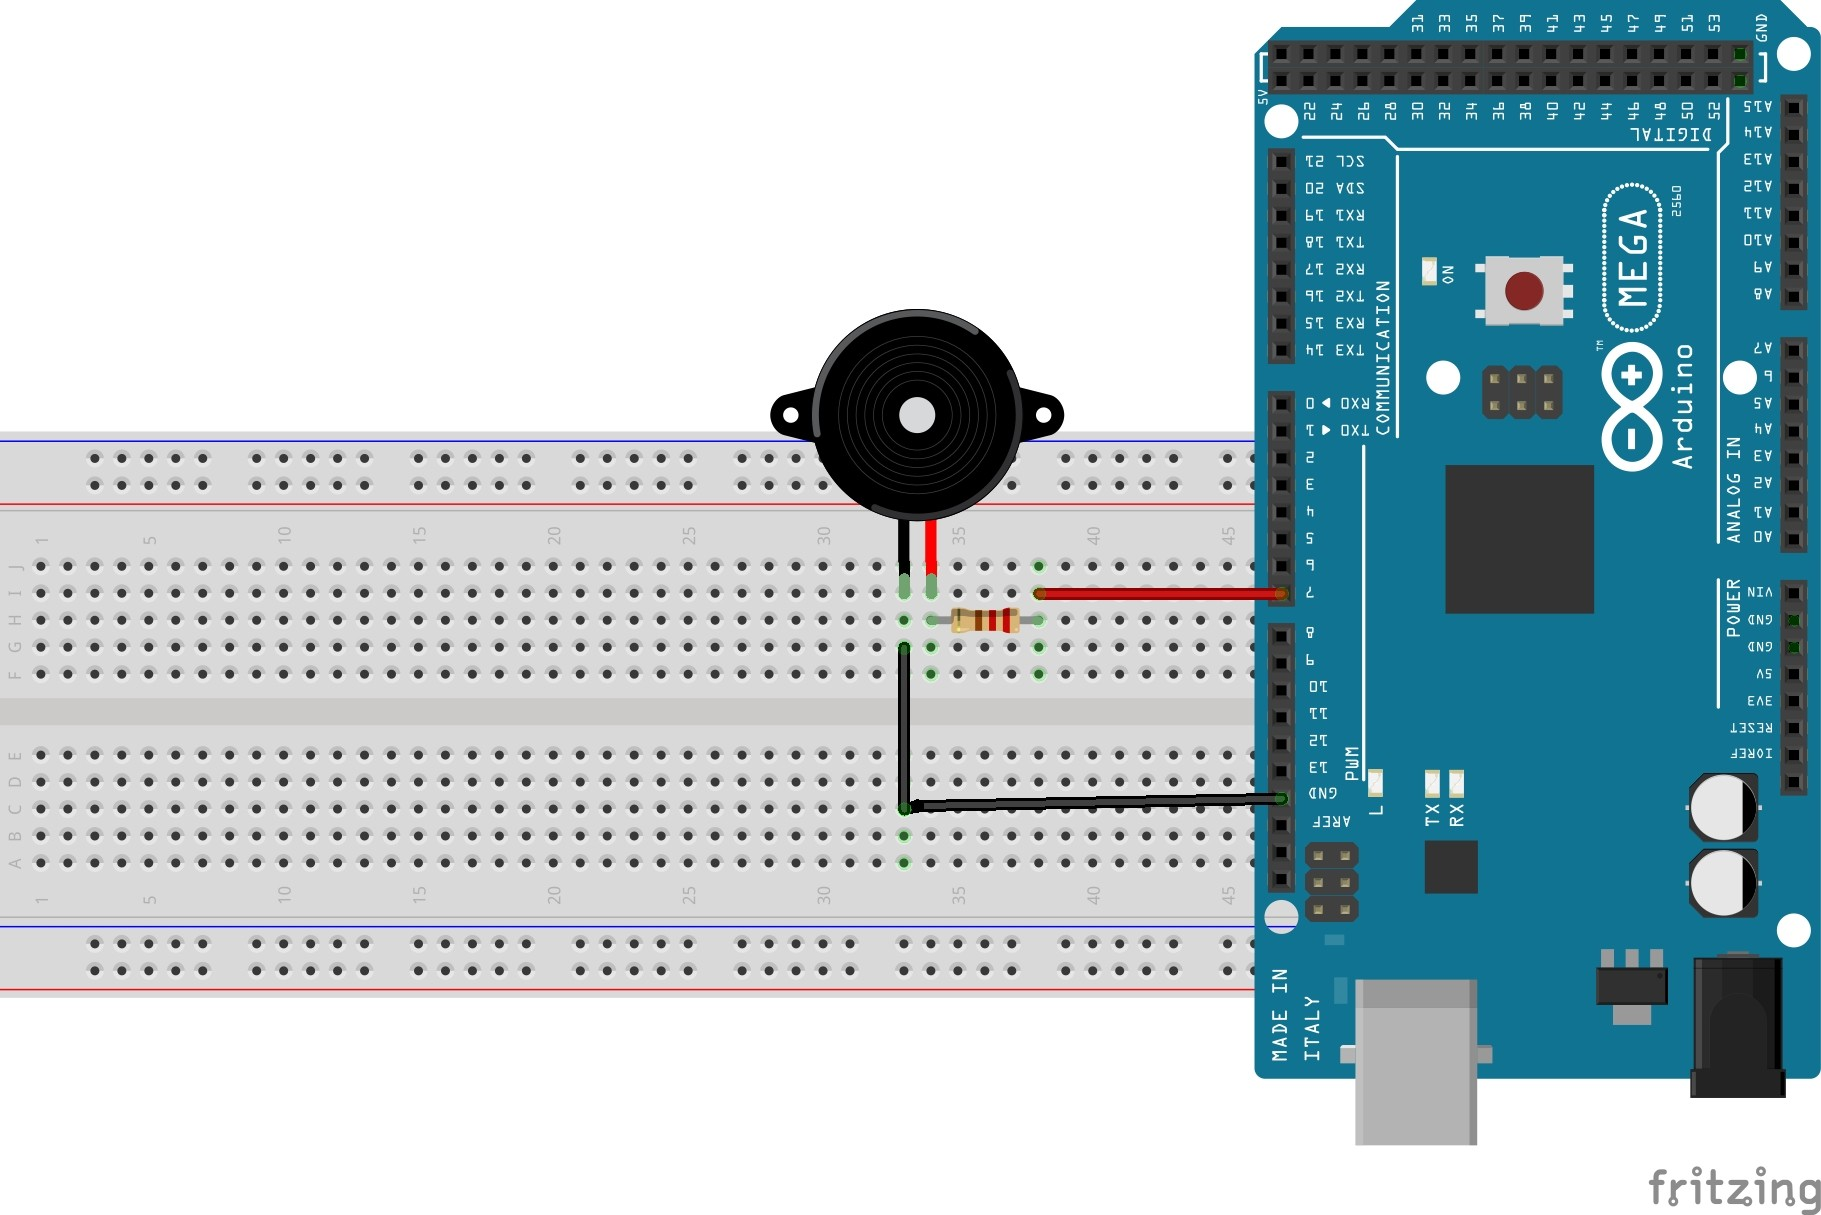
\includegraphics[width=10cm]{sound-fig-2}
  \centering
\end{figure}

Соберём указанную схему на макетной плате, и загрузим нашу программу генерации
звука в Arduino. Не забудьте добавить в тело функции loop вызов нашей функции
\texttt{play\_tone} и настроить цифровой порт, к которому подключен динамик, на
вывод.

Порт, к которому подключен динамик, лучше задать в виде константы
\texttt{SPEAKER\_PIN} в самом начале программы (до функции \texttt{setup}.)

\subsection{Задачи}
\begin{enumerate}
\item Сгенерируйте постоянный сигнал с частотой 261.63 Гц.
\item Сделайте так, чтобы сигнал менялся между 261.63 Гц и 349.23 Гц с частотой
  в 1 секунду. 
\item Модифицируйте систему таким образом, чтобы частота сигнала зависела от
  положения ручки потенциометра. 
\item Сделайте включение звукового сигнала по нажатию кнопки.
\end{enumerate}

Теперь мы можем генерировать звуковой сигнал с нужной нам частотой. Однако, если
мы хотим сгенерировать что-нибудь интересное -- вроде мелодии -- то нам
потребуется использовать вполне определённые частоты. Здесь нам очень кстати
будет хотя бы начальное знание музыкальной теории, но если таких знаний нет --
не беда, разберём по ходу дела.

%%%%%%%%%%%%%%%%%%%%%%%%%%%%%%%%%%%%%%%%%%%%%%%%%%%%%%%%%%%%%%%%%%%%%%%%%%%%%%%%
\section{Теория ритма}

Наш путь в музыку начнётся с разбора теории построения \emph{ритмов}. Думаю,
большинство из нас представляют, что такое ритм -- у многих именно он вызывает
например рефлекс покачивания головой в такт, или машинальное отстукивание ритма
на столешница стола, когда думаем над чем-то.

Чтобы понять, как строится ритм, необходимо знать две простые вещи, о которых мы
сейчас поговорим.

\subsection{Понятие \emph{такта}}

Во-первых, музыкальное произведение делится на отрезки времени, называемые
\emph{тактами} -- как правило одинаковой длительности.\footnote{Музыка отличается
большим разнообразием, и композиторы придумывают всё новые трюки, как получить
желаемое впечатление у слушателя, поэтому здесь мы говорим с некоторыми
допущениями.}

На рисунке ниже показано, как может выглядеть музыкальная композиция из шести
тактов:

\begin{tikzpicture}
  \draw[thick, ->] (0, 0.5) -- (12, 0.5) node[anchor=north west] {t};
  \foreach \x/\n in {0/1, 2/2, 4/3, 6/4, 8/5, 10/6} {
    \draw (\x, 0) -- (\x, 1) -- (\x, 1) node[midway, above] {\n};
  };
\end{tikzpicture}

Протяжённость одного такта во времени определяется быстротой ритма, и про это мы
поговорим позже. Пока можно представить, что один отрезок занимает одну условную
единицу времени. Можете принять эту условую единицу за отрезок времени, удобный
для вашего восприятия -- например, одну секунду.

Во-вторых, эти такты делятся на ещё на более мелкие части, по которым, как по
``ячейкам'', раскладываются различные звуки. Достаточно большая часть музыки
пронизана математикой, и первое математическое, с чем мы столкнёмся -- это
простые дроби. Одним из популярных способов деления такта на части является
$\frac{4}{4}$ или, по-другому называемый ``четыре четверти''. В таком способе
деления такта в него умещается ровно единица некоторого условного времени, про
которое мы говорили выше.\footnote{Существуют более сложные способы деления
такта на части, которые дают суммарное значение меньше или больше единицы -- про
это мы поговорим позднее.}

Если мы поделим каждый такт на четыре части, то получим следующую картину:

\begin{tikzpicture}
  \draw[thick, ->] (0, 0.5) -- (12, 0.5) node[anchor=north west] {t};
  \foreach \x/\n in {0/1, 2/2, 4/3, 6/4, 8/5, 10/6} {
    \draw (\x, 0) -- (\x, 1) -- (\x, 1) node[midway, above] {\n};
  };

  \foreach \x/\n in {0, 0.5, ..., 10} {
    \draw (\x, 0) -- (\x, 0.5);
  };
\end{tikzpicture}

Возьмём отдельный такт и посмотрим на него внимательно:

\begin{tikzpicture}
  \draw[thick] (0, 0.5) -- (8, 0.5) node[anchor=north west] {t};
  \foreach \x/\n in {0/1, 8/2} {
    \draw (\x, 0) -- (\x, 1)  -- (\x, 1) node[midway, above] {\n};
  };

  \foreach \x in {0, 2, ..., 6} {
    \draw (\x, 0) -- (\x, 0.5) node[pos=0.25, right] {$ \frac{1}{4} $};
  };
\end{tikzpicture}

Если просуммируем все части, то снова получим единицу:

\begin{equation}
  \frac{1}{4} + \frac{1}{4} + \frac{1}{4} + \frac{1}{4} = \frac{1}{1}
\end{equation}

На каждую из четвертей можно задать какой-то звук -- пока нам не важно, насколько
он будет музыкальный. Допустим, что три четверти будут звучать с частотой 50Гц,
и одна часть -- с частотой 100Гц:

\begin{tikzpicture}
  \draw[thick] (0, 0.5) -- (8, 0.5) node[anchor=north west] {t};
  \foreach \x/\n in {0/1, 8/2} {
    \draw (\x, 0) -- (\x, 1) -- (\x, 1) node[midway, above] {\n};
  };

  \foreach \x in {0, 2, ..., 6} {
    \draw (\x, 0) -- (\x, 0.5) node[pos=0.25, right] {$ \frac{1}{4} $};
  };

  \foreach \x/\freq in {0/50, 2/50, 4/50, 6/100} {
    \draw (\x, 0) -- (\x, 0.5) node[pos=1.5, right] {\freq Гц};
  };
\end{tikzpicture}

Поздравляю -- мы только что получили с простой ритм. Попробуем запрограммировать
его, беря за длину такта \texttt{T} одну секунду, или 1000000 (миллион)
микросекунд.

Между ``ударами'' необходимо поставить короткую задержку (например, в 100 мс),
чтобы удары одинаковой частоты, идущие один за другим, не сливались в один
долгий звук.

\begin{verbatim}
// Номер порта, куда подключен динамик.
const int SPEAKER = 2;

void setup() {
  pinMode(SPEAKER, OUTPUT);
}

// Функция воспроизведения звука указанной частоты.
void play_tone(int port, float f, long t) {
  const int T = 1000000 / f;
  int d = T / 2;
  int count = t / T;
  for (int i = 0; i < count; i++) {
    digitalWrite(port, HIGH);
    delayMicroseconds(d);
    digitalWrite(port, LOW);
    delayMicroseconds(d);
  }
}

void loop() {
  const long T = 1000000; // Длина такта в микросекундах
  play_tone(SPEAKER, 50, T / 4); // Четверть
  delay(100); // Задержка между звуками
  play_tone(SPEAKER, 50, T / 4); // Четверть
  delay(100);
  play_tone(SPEAKER, 50, T / 4); // Четверть
  delay(100);
  play_tone(SPEAKER, 100, T / 2); // Половина
  delay(100);
}
\end{verbatim}

Можно теперь взять что-то посложнее.

\subsection{Более сложные ритмы}

Возможно некотыре из вас знают такую зажигательную композициюю, как ``We Will
Rock You'' в исполнении группы Queen
(\url{https://www.youtube.com/watch?v=-tJYN-eG1zk}). Данная композиция имеет
чётко выраженный, легко узнаваемый ритм, который можно упрощенно описать как
``два притопа, один прихлоп'', вокруг которого строится вся композиция -- вы сами
можете достаточно легко повторить этот ритм, коротко топая ногой два раза, и
потом делая ``долгий'' хлопок руками.

Структура этого ритма может быть описана следующим набором простых дробей
(\ref{fig:queen-we-will-rock-you-rhythm-1}.) Частоты звуков мы опять же берём
произвольно.

\begin{tikzpicture}
  \label{fig:queen-we-will-rock-you-rhythm-1}
  \draw[thick] (0, 0.5) -- (8, 0.5) node[anchor=north west] {t};
  \foreach \x/\n in {0/1, 8/2} {
    \draw (\x, 0) -- (\x, 1) -- (\x, 1) node[midway, above] {\n};
  };

  \foreach \x in {0, 2} {
    \draw (\x, 0) -- (\x, 0.5) node[pos=0.25, right] {$ \frac{1}{4} $};
  };

  \draw (4, 0) -- (4, 0.5) node[pos=0.25, right] {$ \frac{1}{2} $};

  \foreach \x/\freq in {0/50, 2/50} {
    \draw (\x, 0) -- (\x, 0.5) node[pos=1.5, right] {\freq Гц};
  };
  \draw (4, 0) -- (4, 0.5) node[pos=1.5, right] {100 Гц};
\end{tikzpicture}

Как мы видимо из рисунка \ref{fig:queen-we-will-rock-you-rhythm-1}, деление
такта на части не обязательно должно быть всегда равномерным -- здесь мы получили
две четверти, и одну половину. Суммарно же у нас опять выходит единица (см.
формулу \ref{equation:queen-we-will-rock-you-rhythm-1}.) Попутно вспоминаем, что
для сложения простых дробей нам необходимо их привести к общему знаменателю.

\begin{equation}
  \label{equation:queen-we-will-rock-you-rhythm-1}
  \frac{1}{4} + \frac{1}{4} + \frac{1}{2} = \frac{1}{4} + \frac{1}{4} + \frac{2}{4} = \frac{4}{4} = \frac{1}{1} = 1
\end{equation}

Теперь нам нужно более точно определить, какова длительность целого отрезка
времени, чтобы посчитать длину его частей.

\subsection{Темп музыки}

\emph{Темпом} в музыке скорость исполнения музыки, если говорить упрощенно. В
современной музыке темп измеряется в \emph{ударах в минуту} (буквальный перевод
английского ``Beats per Minute'', сокращённо называемый \emph{BPM}.)

Темп в музыке может задаваться с помощью специального маятника, который
раскачивается из стороны в сторону с равномерной скоростью, делая удары (или
щелчки) в крайних положениях. Такой маятник называется \emph{метрономом}.

\begin{figure}[h]
  \caption{Схематическое изображение механического метронома (источник:
    \url{https://commons.wikimedia.org/wiki/File:Metronome_(PSF).png}).}
  \label{fig:sound-metronome}
  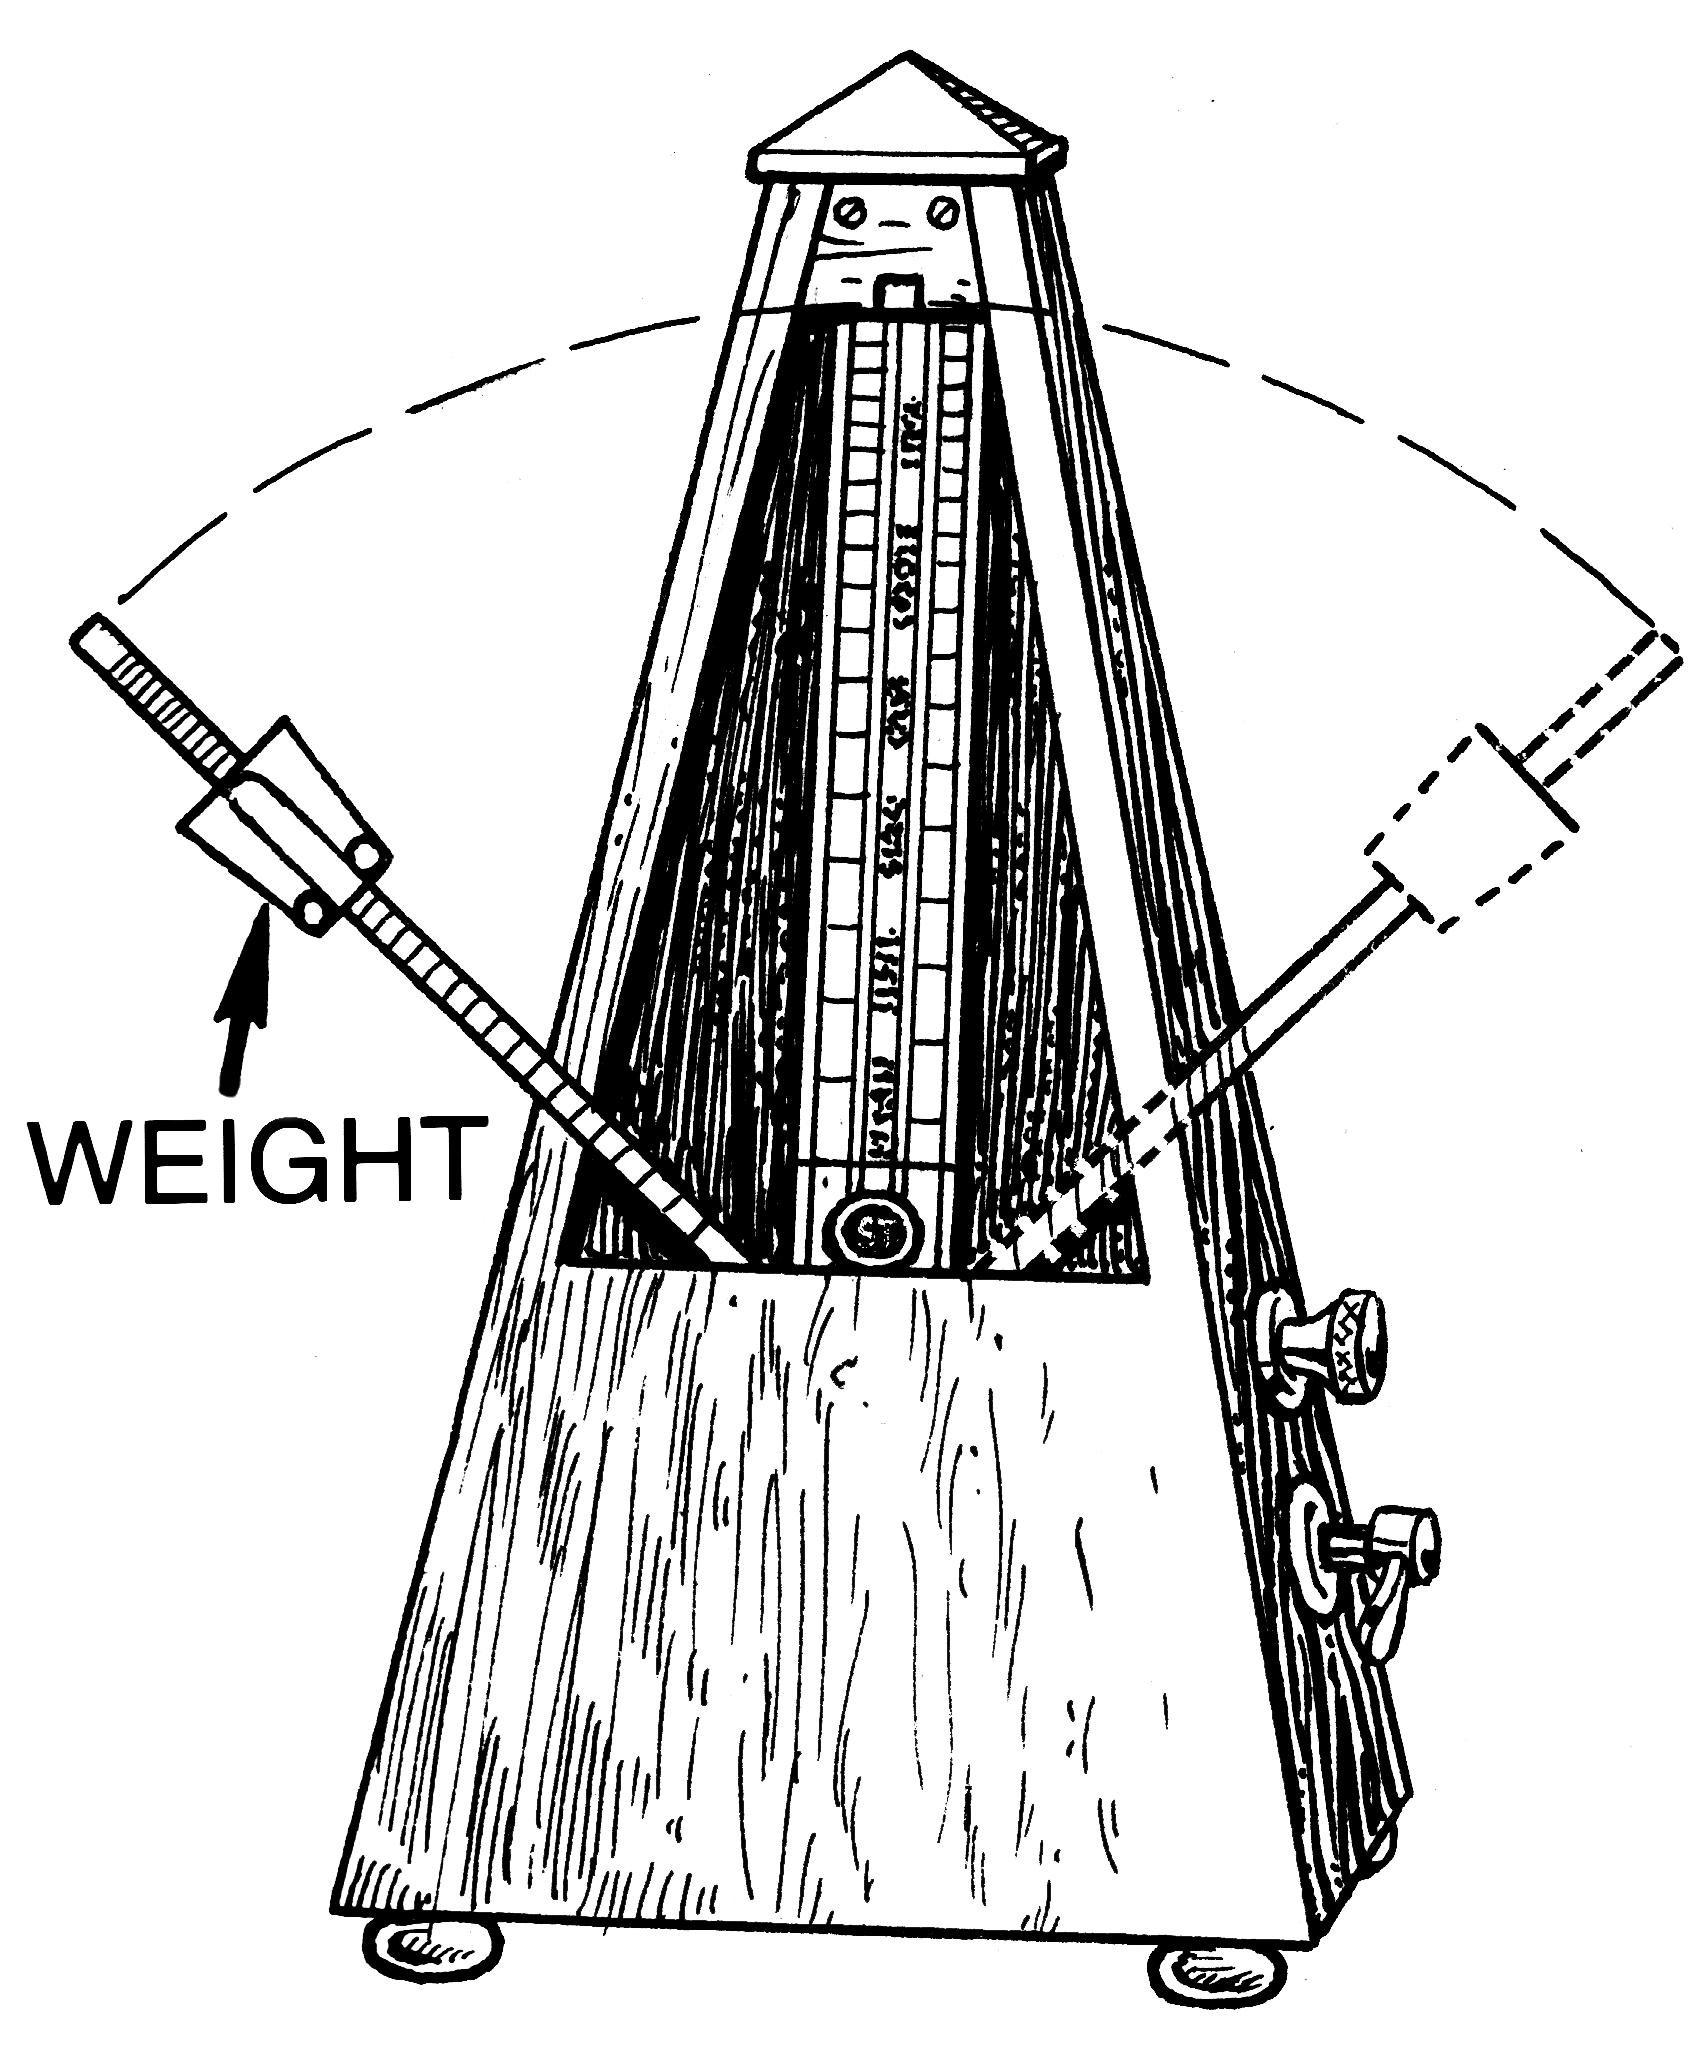
\includegraphics[width=10cm]{Metronome}
  \centering
\end{figure}

В современном мире роль механического маятника часто заменяет специальное
компактное электронное устройство или даже приложение для мобельного телефона,
издающее щелчки через равные промежутки времени с заданной скоростью.

Чем больше ударов в минуту, тем выше темп -- и выше скорость ритма. Примерами BPM
могут служить 60, 80 и 100 ударов в минуту.

Но как связать скорость ритма с делением такта на части? Оказывается,
равномерные удары метронома задают длину одной четверти ($\frac{1}{4}$), на
которые у нас в примерах выше делился такт.

Таким образом, если темп ритма задан в 100 ударов в минуту, то это значит, что в
минуту помещается ровно 100 четвертей.

\begin{tikzpicture}
  \draw[thick] (0, 0.5) -- (10, 0.5) node[anchor=north west] {t};
  \draw (0, -0.5) -- (0, 1.5);
  \draw (10, -0.5) -- (10, 1.5);
  \draw (1, 1.5) node[anchor=north west] {1 минута (60 секунд) / 100 ударов};
  \foreach \x in {0.0, 0.1, 0.2, ..., 10.0} {
    \draw (\x, 0) -- (\x, 1);
  };
\end{tikzpicture}

Расстояние между двумя ударами можно рассчитать по формуле \ref{equation:bpm}.

\begin{equation}
  \label{equation:bpm}
  \frac{\mbox{60 с}}{\mbox{100 ударов}} = \mbox{0.6 с} = \mbox{60 мс} = \mbox{60000 мкс}
\end{equation}

Исходя из формулы \ref{equation:bpm} мы получаем длительность одной четверти в
0.6с. Но для удобства рассчётов мы должны посчитать длину целого такта, а не его
части. Поскольку в такт, который мы рассматриваем в примере, помещается четыре
четверти, для нахождения целого достаточно умножить четверть на четыре (см.
формулу \ref{equation:whole-note-calcualtion-1}).

\begin{equation}
  \label{equation:whole-note-calcualtion-1}
  \frac{1}{4} * 4 = \frac{4}{4} = \frac{1}{1} = 1
\end{equation}

Зная это, можно вывести общую формулу \ref{equation:whole-note-calcualtion-2}
для вычисления длительности целого такта.

\begin{equation}
  \label{equation:whole-note-calcualtion-2}
  \frac{\mbox{60 c}}{\mbox{BPM}} * 4 = \mbox{Длина целого такта}
\end{equation}

Теперь мы можем музыкально точно рассчитать длину звуков, из которых строится
ритм.

Попробуем запрограммировать его.

\begin{verbatim}
// Номер порта, куда подключен динамик.
const int SPEAKER = 2;

void setup() {
  pinMode(SPEAKER, OUTPUT);
}

void play_tone(int port, float f, long t) {
  if (f > 0) {
    const int T = 1000000 / f;
    int d = T / 2;
    int count = t / T;
    for (int i = 0; i < count; i++) {
      digitalWrite(port, HIGH);
      delayMicroseconds(d);
      digitalWrite(port, LOW);
      delayMicroseconds(d);
    }
  } else {
    delay(t / 1000);
  }
}

void loop() {

}
\end{verbatim}

\begin{verbatim}

\end{verbatim}

\section{Октавная система}

Как вы, возможно, знаете, музыка строится из нот -- их всего семь: ``до'',
``ре'', ``ми'', ``фа'', ``соль'', ``ля'', ``си''. Каждой ноте соответствует
определённая частота. Мы уже встречали с вами частоту 261.63 Гц в предыдущей
главе -- так вот, данная частота соответствует ноте ``си''. Ниже в таблице
представлена таблица названий нот и их частот для первой октавы.

\begin{tabular}{p{2cm}|p{3cm}|p{2cm}|p{3cm}}
  № октавы & Слоговое обозначение & Научное обознечение & Частота (Гц) \\
  \hline \hline

  \multirow{7}{*}{4}
  \musicnote{4}{C}{261.630}
  \cline{2-4}
  \musicnote{4}{D}{293.660}
  \cline{2-4}
  \musicnote{4}{E}{329.630}
  \cline{2-4}
  \musicnote{4}{F}{349.230}
  \cline{2-4}
  \musicnote{4}{G}{392.000}
  \cline{2-4}
  \musicnote{4}{A}{440.000}
  \cline{2-4}
  \musicnote{4}{B}{493.880}
  \hline
\end{tabular}

Полный список нот представлен в \nameref{section:appendixA}.

Кроме слогового обозначения нот (от ``до'' до ``си''), в центре можно заметить
столбец с обозначением нот по научной нотации -- мы будем с вами использовать
именно научную нотацию в дальнейшем.

Теперь попробуйте найти по таблице ноту с частотой 349.23 Гц, которую мы
использовали с вами в предыдущей главе --- какая это нота?

Хотя нот всего семь, диапазон частот, используемых в музыке, более обширен --- он
простирается выше и ниже нашей таблицы: от 16.352 Гц до 7902.1 Гц. Как такое
может быть? Дело в том, что данный диапазон частот разделён на 9 групп
(\emph{октав}) и в каждой октаве повторяются все те же семь нот, но уже с
другими частотами.

Для различения нот разных октав обычно явно указывают, к какой октаве та или
иная нота принадлежит (к примеру, нота ``до'' первой октавы.) В научной нотации
октава, к которой принадлежит нота, определяется числом, стоящим после
английской буквы (C, D, E, F, G, A, H или B). К примеру, ``F0'' обозначает ноту
``фа'' самой низкой по частоте октавы, а нота ``F8'' обозначает ноту ``фа'' самой
высокой октавы. Иными словами, чем больше число после буквы, тем выше частота
ноты.

У каждой октавы есть своё имя. Ноты C4-H4 в таблице, которую мы с вами
рассмотрели выше, относятся к первой октаве -- она находится в центре частотного
диапазона. Ноты C5-H5 относятся ко второй октаве, которая -- как можно догадаться
-- идёт после первой. А вот октава, которая идёт перед первой, называется малой
октавой, и ноты, которые в неё входят, именуются C3-H3 в научной нотации.

Одинаковые ноты в разных октавах звучат на слух очень похоже -- например, нота C4
звучит похоже на ноту C3, только выше по частоте. Если посмотреть на частоты этих
двух нот, то можно заметить, что нота C4 ("до" первый октавы) в два раза выше по
39частоте, чем нота C3 ("до" малой октавы). Именно это свойство и лежит в основе
октавной системы, используемый в музыке.

Если вам интересно покопать глубже этот вопрос, то рекомендуем ознакомиться с
таблицей в \nameref{section:appendixA} -- там можно посмотреть частоты нот для
всех октав, что может пригодиться при программировании мелодий на Arduino.

\section{Программирование простых мелодий}

Для того, чтобы запрограммировать мелодию, нам потребуется узнать ноты, из
которых состоит данная мелодия, и их порядок. Как правило, эта информация
записывается в виде нотной записи -- но если вы ещё не умеете читать нотную
запись, то можно найти мелодии в упрощенной записи, где используется буквенная
(научная) нотация. К примеру, возьмём мелодию ``Twinkle, Twinkle, Little
Star'' \footnote{\url{https://ru.wikipedia.org/wiki/Twinkle,_Twinkle,_Little_Star}}
-- английскую колыбельную:

\begin{figure}[h]
  \caption{Мелодия ``Twinkle, Twinkle, Little Star''.}
  \label{fig:sound-fig-3}
  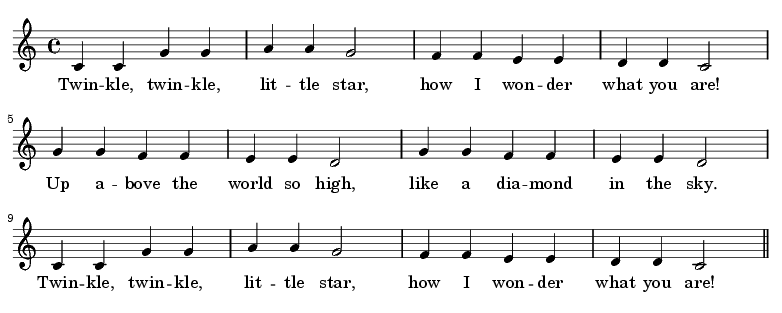
\includegraphics[width=10cm]{twinkle-twinkle-little-star}
  \centering
\end{figure}

Это относительно простая мелодия, однако без знания нотной записи прочитать её
будет проблематично. Мы не будем сейчас вдаваться в изучение нотной грамоты;
вместо этого ниже представлена запись этой мелодии в научной нотации:

\begin{verbatim}
C4 C4 G4 G4 A4 A4 G4
F4 F4 E4 E4 D4 D4 C4
G4 G4 F4 F4 E4 E4 D4
G4 G4 F4 F4 E4 E4 D4
C4 C4 G4 G4 A4 A4 G4
\end{verbatim}

Для того, чтобы запрограммировать данную мелодию, удобно в начале программы
объявить каждую ноту в виде константы. Каждая константа будет хранить частоту
звука:\footnote{Имена констант обычно пишутся заглавными буквами, т.е.
правильнее было бы именовать эти константы C4, D4, E4 и т.д. Однако мы
используем здесь буквы в нижнем регистре, чтобы избежать конфликтов имён с
константами, которые уже есть в Arduino (к примеру, A4.)}

\begin{verbatim}
const long c4 = 261.63;
const long d4 = 293.66;
// И так далее
\end{verbatim}

Как только мы объявили все необходимые константы (для ``Twinkle, Twinkle, Little
Star'' нам потребуются только ноты из первой октавы), то запрограммировать
мелодию не составит труда. Однако, как мы уже говорили, большинство задач может
быть решено несколькими способами, и некоторые способы лучше (можно сказать,
красивее), чем другие.

Первое решение, которое может прийти на ум -- это вызвать нашу функцию
\texttt{play\_tone} для каждой ноты, в нужном нам порядке:

\begin{verbatim}
const long N = 1000000; // 1 секунда в микросекундах
void loop() {
  play_tone(SPEAKER_PIN, c4, N);
  delay(100);
  play_tone(SPEAKER_PIN, c4, N);
  delay(100);
  play_tone(SPEAKER_PIN, g4, N);
  delay(100);
  play_tone(SPEAKER_PIN, g4, N);
  delay(100);
  // и так далее
}
\end{verbatim}

Но данное решение является не совсем оптимальным с точки зрения количества кода,
которое необходимо напмсать. Решением данной проблемы является использование
\emph{массивов}.

\section{Использование массива для программирования мелодии}



\subsection{Задачи}
\begin{itemize}
\item Добавьте паузы между воспроизведением нот.
\item Попробуйте сделать управление скоростью воспроизведения мелодии с
  использованием потенциометра.
\item Сделайте ``светомузыку'' -- модифицируйте программу и схему на макетной плате
  таким образом, чтобы на каждую из семи нот загорался свой светодиод. После
  воспроизведения ноты светодиод должен гаснуть.
\end{itemize}

\section{Приложение А}
\label{section:appendixA}
\begin{longtable}{crll}
  № октавы & Слоговое обозначение & Научное обознечение & Частота (Гц) \\
  \hline \hline

  \multirow{7}{*}{0}
  \musicnote{0}{C}{16.352}
  \cline{2-4}
  \musicnote{0}{D}{18.354}
  \cline{2-4}
  \musicnote{0}{E}{20.602}
  \cline{2-4}
  \musicnote{0}{F}{21.827}
  \cline{2-4}
  \musicnote{0}{G}{24.500}
  \cline{2-4}
  \musicnote{0}{A}{27.500}
  \cline{2-4}
  \musicnote{0}{B}{30.868}
  \hline

  \multirow{7}{*}{1}
  \musicnote{1}{C}{32.703}
  \cline{2-4}
  \musicnote{1}{D}{36.708}
  \cline{2-4}
  \musicnote{1}{E}{41.203}
  \cline{2-4}
  \musicnote{1}{F}{43.654}
  \cline{2-4}
  \musicnote{1}{G}{48.999}
  \cline{2-4}
  \musicnote{1}{A}{55.000}
  \cline{2-4}
  \musicnote{1}{B}{61.735}
  \hline

  \multirow{7}{*}{2}
  \musicnote{2}{C}{65.406}
  \cline{2-4}
  \musicnote{2}{D}{73.416}
  \cline{2-4}
  \musicnote{2}{E}{82.407}
  \cline{2-4}
  \musicnote{2}{F}{87.307}
  \cline{2-4}
  \musicnote{2}{G}{97.999}
  \cline{2-4}
  \musicnote{2}{A}{110.000}
  \cline{2-4}
  \musicnote{2}{B}{123.470}
  \hline

  \multirow{7}{*}{3}
  \musicnote{3}{C}{130.810}
  \cline{2-4}
  \musicnote{3}{D}{146.830}
  \cline{2-4}
  \musicnote{3}{E}{164.810}
  \cline{2-4}
  \musicnote{3}{F}{174.610}
  \cline{2-4}
  \musicnote{3}{G}{196.000}
  \cline{2-4}
  \musicnote{3}{A}{220.000}
  \cline{2-4}
  \musicnote{3}{B}{246.940}
  \hline

  \multirow{7}{*}{4}
  \musicnote{4}{C}{261.630}
  \cline{2-4}
  \musicnote{4}{D}{293.660}
  \cline{2-4}
  \musicnote{4}{E}{329.630}
  \cline{2-4}
  \musicnote{4}{F}{349.230}
  \cline{2-4}
  \musicnote{4}{G}{392.000}
  \cline{2-4}
  \musicnote{4}{A}{440.000}
  \cline{2-4}
  \musicnote{4}{B}{493.880}
  \hline

  \multirow{7}{*}{5}
  \musicnote{5}{C}{523.250}
  \cline{2-4}
  \musicnote{5}{D}{587.320}
  \cline{2-4}
  \musicnote{5}{E}{659.260}
  \cline{2-4}
  \musicnote{5}{F}{698.460}
  \cline{2-4}
  \musicnote{5}{G}{783.990}
  \cline{2-4}
  \musicnote{5}{A}{880.000}
  \cline{2-4}
  \musicnote{5}{B}{987.770}
  \hline

  \multirow{7}{*}{6}
  \musicnote{6}{C}{1046.500}
  \cline{2-4}
  \musicnote{6}{D}{1174.700}
  \cline{2-4}
  \musicnote{6}{E}{1318.500}
  \cline{2-4}
  \musicnote{6}{F}{1396.900}
  \cline{2-4}
  \musicnote{6}{G}{1568.000}
  \cline{2-4}
  \musicnote{6}{A}{1760.000}
  \cline{2-4}
  \musicnote{6}{B}{1975.500}
  \hline

  \multirow{7}{*}{7}
  \musicnote{7}{C}{2093.000}
  \cline{2-4}
  \musicnote{7}{D}{2349.300}
  \cline{2-4}
  \musicnote{7}{E}{2637.000}
  \cline{2-4}
  \musicnote{7}{F}{2793.800}
  \cline{2-4}
  \musicnote{7}{G}{3136.000}
  \cline{2-4}
  \musicnote{7}{A}{3520.000}
  \cline{2-4}
  \musicnote{7}{B}{3951.100}
  \hline

  \multirow{7}{*}{8}
  \musicnote{8}{C}{4186.000}
  \cline{2-4}
  \musicnote{8}{D}{4698.600}
  \cline{2-4}
  \musicnote{8}{E}{5274.000}
  \cline{2-4}
  \musicnote{8}{F}{5587.700}
  \cline{2-4}
  \musicnote{8}{G}{6271.900}
  \cline{2-4}
  \musicnote{8}{A}{7040.000}
  \cline{2-4}
  \musicnote{8}{B}{7902.100}
  \hline

  \caption{Октавная система}
  \label{table:octaveList}

\end{longtable}


\section{Список сокращений}
\begin{acronym}
  \acro{ШИМ}{Широтно-импульсная модуляция}
\end{acronym}
\end{document}

